\documentclass[10pt]{article}
\usepackage[letterpaper,text={6.5in,8.7in},centering]{geometry}
\usepackage{amssymb,amsmath,times,url,subfigure,graphicx,theorem,alltt,eepic,epic,color,tikz}
%\usepackage[pdftex,urlcolor=blue,pdfpagemode=none,pdfstartview=FitH]{hyperref}

%% url smaller font.
\makeatletter
\def\url@leostyle{%
  \@ifundefined{selectfont}{\def\UrlFont{\sf}}{\def\UrlFont{\small\ttfamily}}}
\makeatother
\urlstyle{leo}

%\usepackage[all,import]{xy}

\newcommand{\norm}[1]{\ensuremath{\left\| #1 \right\|}}
\newcommand{\abs}[1]{\ensuremath{\left| #1 \right|}}
\newcommand{\bracket}[1]{\ensuremath{\left[ #1 \right]}}
\newcommand{\braces}[1]{\ensuremath{\left\{ #1 \right\}}}
\newcommand{\parenth}[1]{\ensuremath{\left( #1 \right)}}
\newcommand{\ip}[1]{\ensuremath{\langle #1 \rangle}}
\newcommand{\refeqn}[1]{(\ref{eqn:#1})}
\newcommand{\reffig}[1]{Fig. \ref{fig:#1}}
\newcommand{\tr}[1]{\mbox{tr}\ensuremath{\negthickspace\bracket{#1}}}
\newcommand{\deriv}[2]{\ensuremath{\frac{\partial #1}{\partial #2}}}
\newcommand{\SO}{\ensuremath{\mathrm{SO(3)}}}
\newcommand{\T}{\ensuremath{\mathrm{T}}}
\newcommand{\so}{\ensuremath{\mathfrak{so}(3)}}
\newcommand{\SE}{\ensuremath{\mathrm{SE(3)}}}
\newcommand{\se}{\ensuremath{\mathfrak{se}(3)}}
\renewcommand{\Re}{\ensuremath{\mathbb{R}}}
\renewcommand{\S}{\ensuremath{\mathbb{S}}}
\newcommand{\aSE}[2]{\ensuremath{\begin{bmatrix}#1&#2\\0&1\end{bmatrix}}}
\newcommand{\ase}[2]{\ensuremath{\begin{bmatrix}#1&#2\\0&0\end{bmatrix}}}
\newcommand{\D}{\ensuremath{\mathbf{D}}}
\newcommand{\pair}[1]{\ensuremath{\left\langle #1 \right\rangle}}
\newcommand{\met}[1]{\ensuremath{\langle\!\langle #1 \rangle\!\rangle}}
\newcommand{\Ad}{\ensuremath{\mathrm{Ad}}}
\newcommand{\ad}{\ensuremath{\mathrm{ad}}}
\newcommand{\g}{\ensuremath{\mathfrak{g}}}

\renewcommand{\baselinestretch}{1.2}
\date{}

\renewcommand{\thesubsection}{\arabic{subsection}. }
\renewcommand{\thesubsubsection}{\arabic{subsection}.\arabic{subsubsection} }

\theoremstyle{plain}\theorembodyfont{\normalfont}
\newtheorem{prob}{Problem}[section]
%\renewcommand{\theprob}{\arabic{section}.\arabic{prob}}
\renewcommand{\theprob}{\arabic{prob}}

\newenvironment{subprob}%
{\renewcommand{\theenumi}{\alph{enumi}}\renewcommand{\labelenumi}{(\theenumi)}\begin{enumerate}}%
{\end{enumerate}}%

\newenvironment{matlab}
{\begin{alltt}\small\renewcommand{\baselinestretch}{1.2}\selectfont}%
{\end{alltt}}

\newcommand*\circled[1]{%
  \tikz[baseline=(C.base)]\node[draw,circle,inner sep=0.5pt](C) {#1};\!
}

\begin{document}

\pagestyle{empty}
\section*{MAE3145: Solution for Homework 5, Question 3}
%\vspace*{-0.4cm}
%\noindent{Due date: November 19, 2012}%\\%\vspace*{0.5cm}

%\begin{prob}
%Consider a reentry vehicle at the point $A$ on a circular orbit around the Earth. We wish to design a reentry orbit such that the vehicle arrives at $B$ along a trajectory tangent to the surface of the Earth at $B$, i.e. the point $B$ is the periapsis of the reentry orbit. 
%
%\definecolor{gray}{rgb}{0.1, 0.1, 0.1}
%\centerline{
%\setlength{\unitlength}{1.5em}\centering\small
%\begin{picture}(10,10)(-5,-5)
%{\filltype{shade}\put(0,0){\circle*{4}}}
%\put(0,0){\vector(1,0){4.8}}
%\put(0,0){\vector(0,1){4.8}}
%\put(0,0){\circle{8}}
%\put(-3.4641,-2){\circle*{0.15}}
%\put(2,0){\circle*{0.15}}
%\put(-3.9,-2.5){$A$}
%\put(2.1,-0.5){$B$}
%\put(5.0,-0.4){$\hat x$}
%\put(0.3,4.5){$\hat y$}
%%\linethickness{8pt}
%\put(-0.5,-1.0){Earth}
%\end{picture}}
%\vspace*{-0.3cm}
%%
%\noindent The initial circular orbit is referred to as Orbit 1, and the reentry orbit is referred to as Orbit 2. We do not consider the atmospheric drag effects. Assume that
%\begin{gather*}
%R_1 = 7000\,\mathrm{km},\quad R_E=6378\,\mathrm{km},\quad \mu=398600\,\mathrm{km^3/s^2},\quad \theta_A=210^\circ.
%\end{gather*}
%Recall that the velocity vector of a mass located at $\theta$ on an orbit with $h,e$ is given by
%\begin{align*}
%\vec v = \frac{\mu}{h} [-\sin\theta \hat x + (e+\cos\theta)\hat y].
%\end{align*}
%
%\begin{subprob}
%\item Find the velocity vector $\vec v_{A_1}$ of the reentry vehicle at the point $A$ on Orbit 1.
%\item Find the eccentricity $e_2$ and the specific angular momentum $h_2$ of Orbit 2.
%\item Find the velocity vector $\vec v_{A_2}$ of the reentry vehicle at the point $A$ on Orbit 2.
%\item Find the required velocity change $\vec v_A$ at the point $A$.
%\item Find the resulting velocity $\vec v_{B_2}$ of the reentry vehicle at the surface of the Earth.
%\end{subprob}
%\end{prob}
%
%\begin{prob}
%We solve Exercise 6.21 of the textbook. Two spacecraft are on the same elliptic orbit with $r_p=8000\,\mathrm{km}$, $r_a=13000\,\mathrm{km}$. Currently, Spacecraft 1 is at the point $P$ ($\theta_P=0$), and Spacecraft 2 is at the point $C$ ($\theta_C=30^\circ$). We will find the velocity change for Spacecraft 1 to intercept and rendezvous with Spacecraft 2 at the point $D$ ($\theta_D=90^\circ$).
%
%\vspace*{0.2cm}
%\centerline{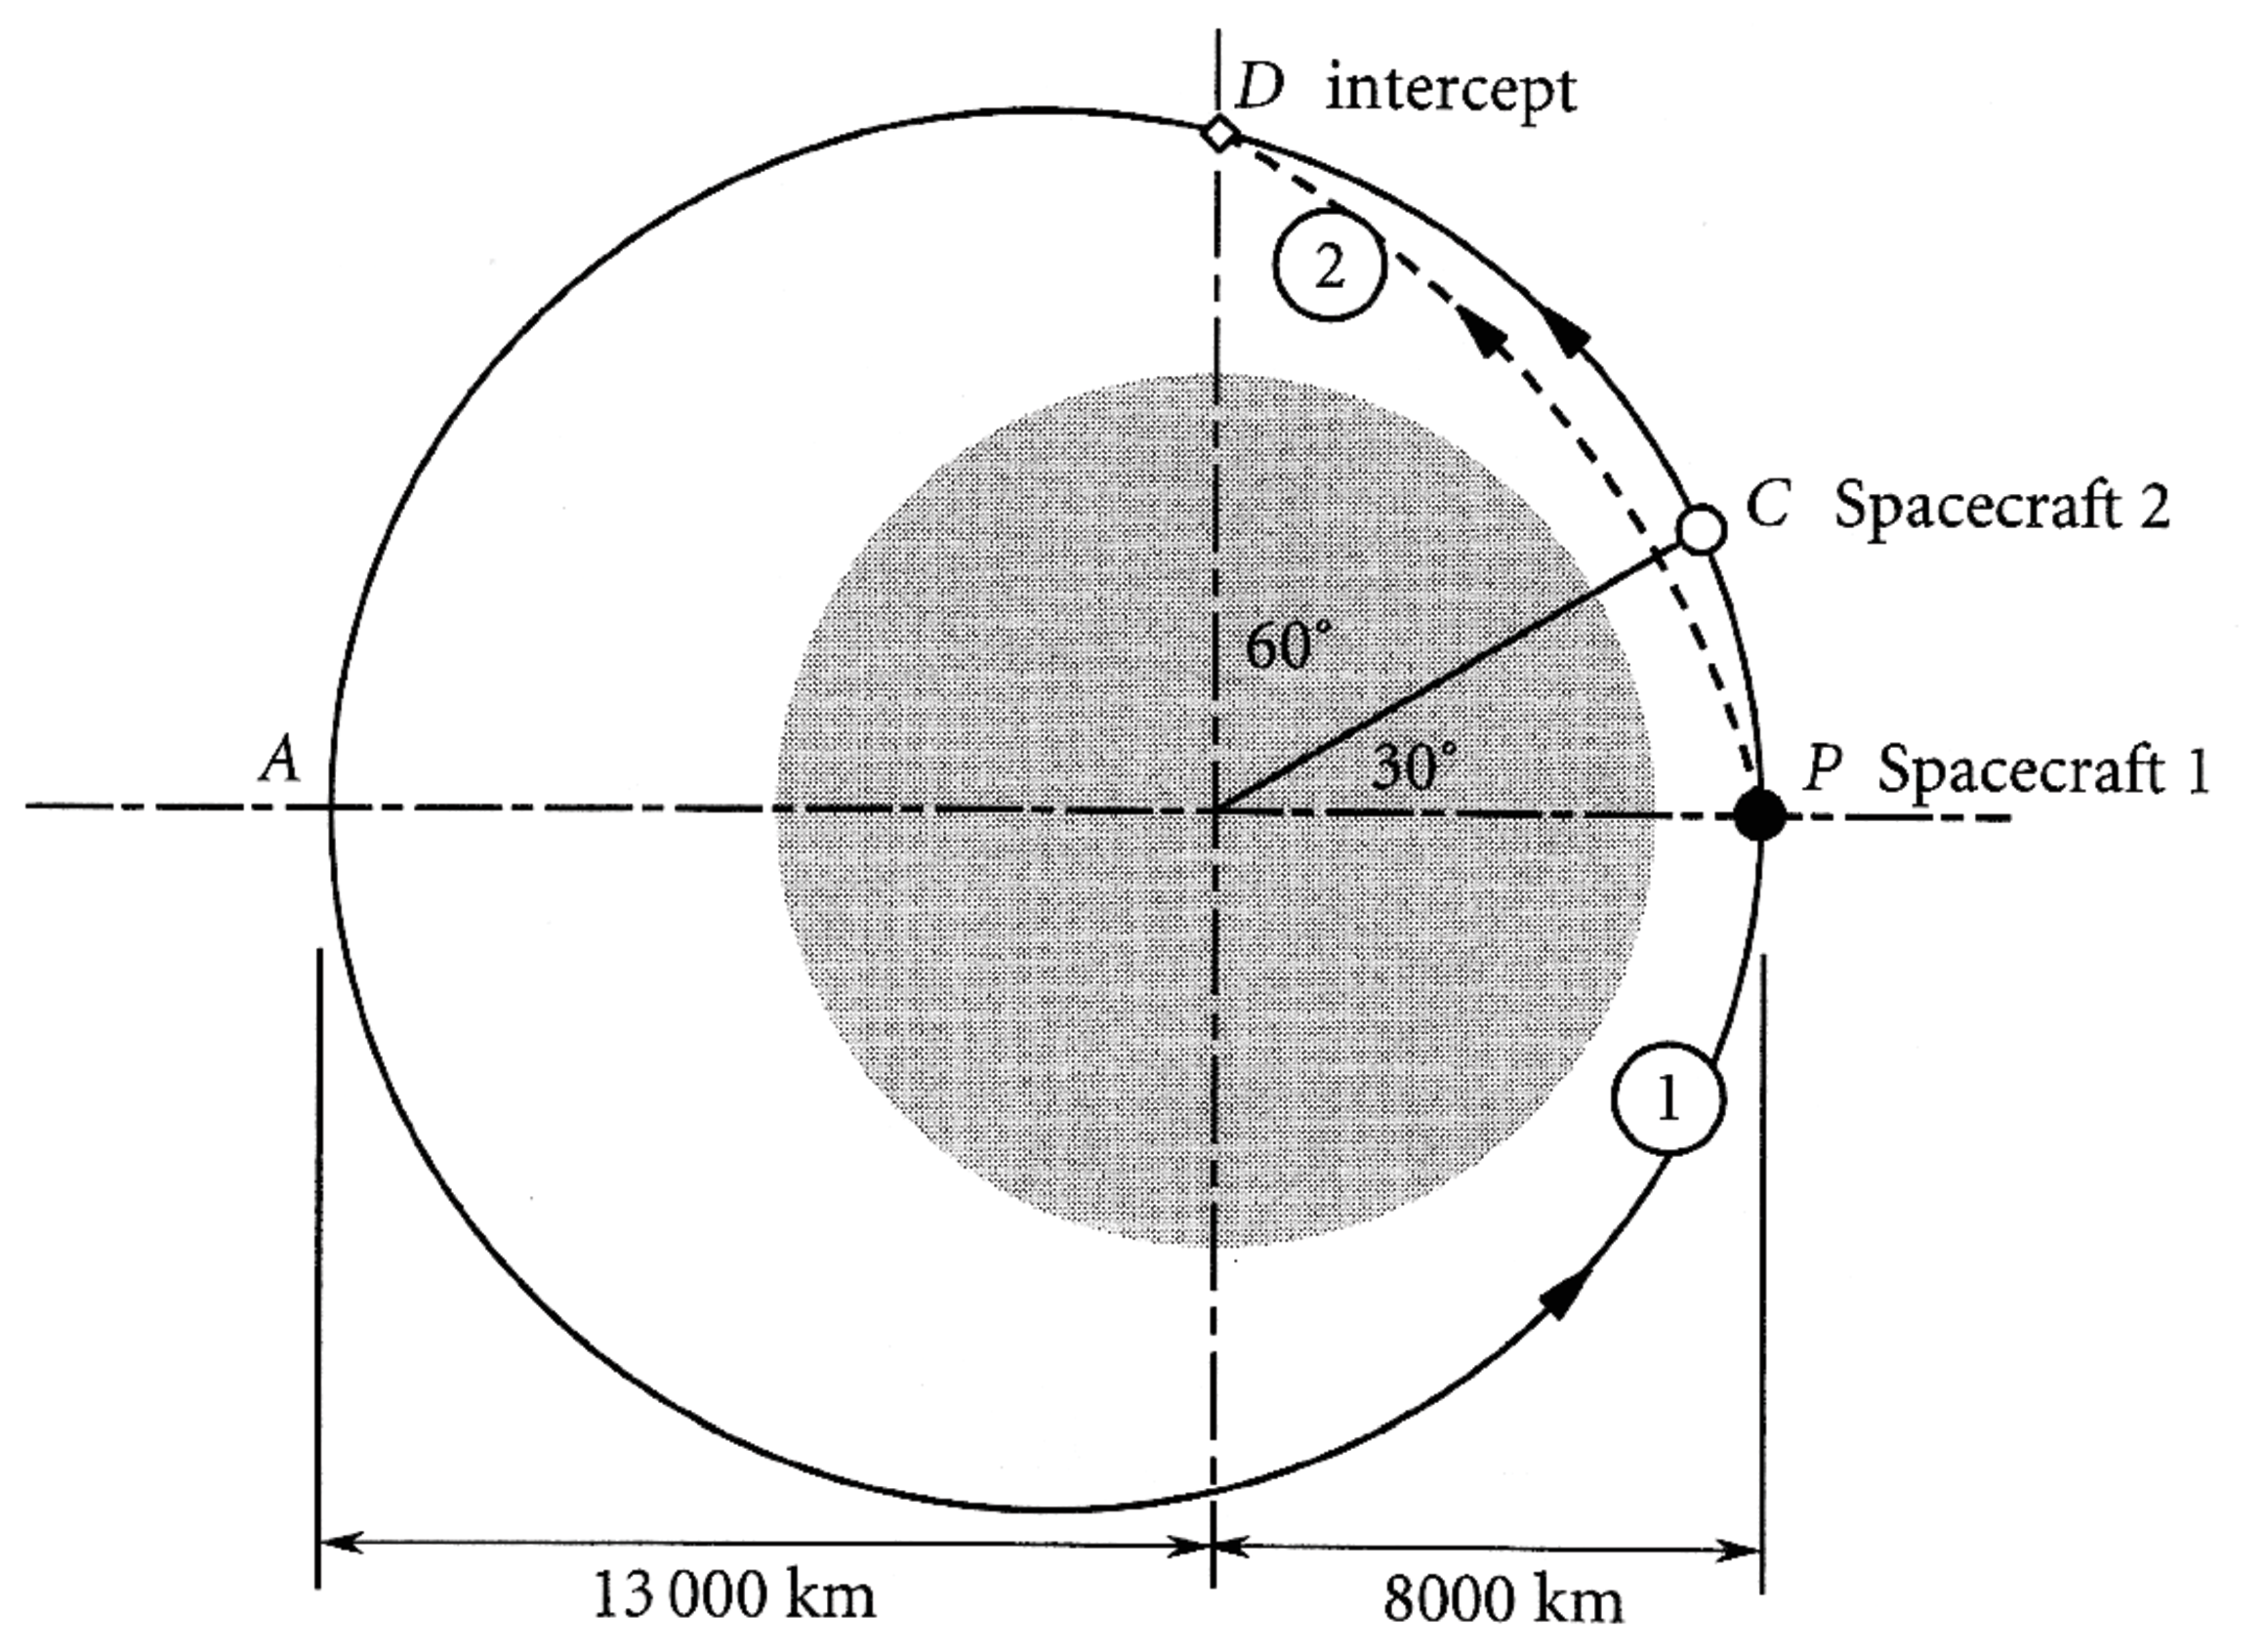
\includegraphics[width=0.45\textwidth]{prob2.eps}}
%
%Recall that the position vector of a mass located at $\theta$ on an orbit with $h,e$ is given by
%\begin{align*}
%\vec r = r [\cos\theta \hat x + \sin\theta\hat y],\qquad \text{where}\quad r=\frac{h^2}{\mu}\frac{1}{1+e\cos\theta}.
%\end{align*}
%
%
%\begin{subprob}
%\item Find the position vector $\vec r_P$ and the velocity vector $\vec v_{P_1}$ of Spacecraft 1 at the point $P$ of Orbit 1.
%\item Find the position vector $\vec r_D$ and the velocity vector $\vec v_{D_1}$ of Spacecraft 1 at the point $D$ of Orbit 1.
%\item Show that the time required for Spacecraft 2 to move from $C$ to $D$ is $t_{CD}=1.3304\times 10^3$ seconds.
%\item The Matlab function \texttt{LambertProb.m} posted at Black Board finds the solution of a Lambert problem. It has the following input and output variables: 
%
%\begin{matlab}
%function [vA_vec vB_vec]=LambertProb(rA_vec,rB_vec,tAB,mu)
%% Input 1: rA_vec the position vector to the initial point A
%% Input 2: rB_vec the position vector to the terminal point B
%% Input 3: tAB transfer time from A to B
%% Input 4: mu gravitational parameter
%% Output 1: vA_vec the velocity vector at A on the transfer orbit
%% Output 2: vB_vec the velocity vector at B on the transfer orbit
%\end{matlab}
%Using this function, find the velocity vector $\vec v_{P_2}$ and $\vec v_{D_2}$ of Spacecraft 1 on the transfer orbit, Orbit 2.
%
%\item Find the required velocity change $\Delta \vec v_P$ and $\Delta \vec v_D$ of Spacecraft 1 at $P$ and $D$
%\item Show that the total velocity change is $\Delta v_{total}=6.239\,\mathrm{km/s}$.
%
%\end{subprob}
%\end{prob}

\setcounter{prob}{2}
\begin{prob}
Consider the following two elliptic orbits that have the same eccentricity $e$ and specific angular momentum $h$. The gravitational parameter is given by $\mu$.

\begin{subprob}
\item Assume that $\vec h_1 = \vec h_2 = h \hat z$, i.e. in both orbits, the spacecraft rotates counter-clockwise. Find the magnitude of the required velocity change at $A$ on Orbit 1 to transfer the spacecraft to Orbit 2.

\paragraph{Solution:} The velocity vector of the $i$-th spacecraft can be written as
\begin{align*}
\vec v_i = \frac{\mu}{h} [-\sin\theta_i \hat x_i + (e+\cos\theta_i)\hat y_i],
\end{align*}
where $\theta_i$ is measured along the direction of movement from the periapsis, $\hat x_i$ points toward the periapsis, and $\hat y_i$ points toward $\hat h_i\times \hat x_i$, or $\theta_i=90^\circ$. The unit-vectors $\hat x_i,\hat y_i$ and the true anomaly $\theta_i$ for both spacecraft are illustrated as follows:

\centerline{
\setlength{\unitlength}{1.8em}\centering\small
\begin{picture}(20,6.5)(-10,-3)
\put(0,0){\vector(1,0){7}}
\put(0,0){\vector(0,1){3}}
\put(-2,0){\ellipse{7}{4}}
\put(0,1.62){\circle*{0.15}}
\put(0.1,1.9){$A$}
\put(0,0){\circle*{0.6}}
\put(-3.2,-2.5){Orbit 1}
\put(6.5,-0.5){$\hat x_1=\hat x$}
\put(0.2,2.8){$\hat y_1=\hat y$}
\put(-2.5,2){\vector(-1,0){0}}
\put(-2.1,-2){\vector(1,0){0}}
\put(1.5,0){\circle*{0.15}}
\put(1.6,-0.5){{$P_1$}}
\put(-6,-2.5){\textcolor{black}{$\theta_1=90^\circ$}}
\color{blue}
\put(2.1,2){\vector(-1,0){0}}
\put(2.5,-2){\vector(1,0){0}}
\put(-7.5,-0.5){$\hat x_2=-\hat x$}
\put(0.2,-3.2){$\hat y_2=-\hat y$}
\put(0,0){\vector(-1,0){7}}
\put(0,0){\vector(0,-1){3}}
\put(2,0){\ellipse{7}{4}}
\put(-1.5,0){\circle*{0.15}}
\put(-2.0,-0.5){\textcolor{blue}{$P_2$}}
\put(1.6,-2.5){\textcolor{blue}{Orbit 2}}
\put(4,-2.5){\textcolor{blue}{$\theta_2=270^\circ$}}
\end{picture}}
Therefore, the velocity vectors are given by
\begin{align*}
\vec v_1 & = \frac{\mu}{h} [-\sin \theta_1 \hat x_1 + (e+\cos \theta_1)\hat y_1]
=\frac{\mu}{h} [-\sin 90^\circ \hat x + (e+\cos 90^\circ)\hat y]=\frac{\mu}{h}[-\hat x + e\hat y],\\
\vec v_2 & = \frac{\mu}{h} [-\sin \theta_2 \hat x_2 + (e+\cos \theta_2)\hat y_2]
=\frac{\mu}{h} [-\sin 270^\circ (-\hat x) + (e+\cos 270^\circ))(-\hat y)]=\frac{\mu}{h}[-\hat x -e\hat y],\\
\Delta \vec v & = \vec v_2 -\vec v_1 = -\frac{2\mu e}{h}\hat y.
\end{align*}


\item Assume that $\vec h_1 = -\vec h_2 = h \hat z$, i.e. the spacecraft rotates counter-clockwise on Orbit 1, and it rotates clockwise on Orbit 2. Find the magnitude of the required velocity change at $A$ on Orbit 1 to transfer the spacecraft to Orbit 2.

\paragraph{Solution:} Similarly, we have

\centerline{
\setlength{\unitlength}{1.8em}\centering\small
\begin{picture}(20,6.5)(-10,-3)
\put(0,0){\vector(1,0){7}}
\put(0,0){\vector(0,1){3}}
\put(-2,0){\ellipse{7}{4}}
\put(0,1.62){\circle*{0.15}}
\put(0.1,1.9){$A$}
\put(0,0){\circle*{0.6}}
\put(-3.2,-2.5){Orbit 1}
\put(6.5,-0.5){$\hat x_1=\hat x$}
\put(0.2,2.8){$\hat y_1=\hat y$\;\textcolor{blue}{$=\hat y_2$}}
\put(-2.5,2){\vector(-1,0){0}}
\put(-2.1,-2){\vector(1,0){0}}
\put(1.5,0){\circle*{0.15}}
\put(1.6,-0.5){{$P_1$}}
\put(-6,-2.5){\textcolor{black}{$\theta_1=90^\circ$}}
\color{blue}
\put(2.5,2){\vector(1,0){0}}
\put(2.1,-2){\vector(-1,0){0}}
\put(-7.5,-0.5){$\hat x_2=-\hat x$}
\put(0,0){\vector(-1,0){7}}
\put(2,0){\ellipse{7}{4}}
\put(-1.5,0){\circle*{0.15}}
\put(-2.0,-0.5){\textcolor{blue}{$P_2$}}
\put(1.6,-2.5){\textcolor{blue}{Orbit 2}}
\put(4,-2.5){\textcolor{blue}{$\theta_2=90^\circ$}}
\end{picture}}
Therefore, the velocity vectors are given by
\begin{align*}
\vec v_1 & = \frac{\mu}{h} [-\sin \theta_1 \hat x_1 + (e+\cos \theta_1)\hat y_1]
=\frac{\mu}{h} [-\sin 90^\circ \hat x + (e+\cos 90^\circ)\hat y]=\frac{\mu}{h}[-\hat x + e\hat y],\\
\vec v_2 & = \frac{\mu}{h} [-\sin \theta_2 \hat x_2 + (e+\cos \theta_2)\hat y_2]
=\frac{\mu}{h} [-\sin 90^\circ (-\hat x) + (e+\cos 90^\circ)\hat y]=\frac{\mu}{h}[\hat x +e\hat y],\\
\Delta \vec v & = \vec v_2 -\vec v_1 = \frac{2\mu }{h}\hat x.
\end{align*}

\end{subprob}
\end{prob}
\end{document}

